\documentclass[14pt]{article}
\usepackage[utf8]{inputenc}
\usepackage[english]{babel}
\usepackage{amsmath, amssymb}
\usepackage{geometry}
\usepackage{graphicx}
\usepackage{xcolor}
\usepackage{hyperref}
\usepackage{tasks}
\usepackage{tcolorbox}
\tcbuselibrary{skins, breakable, theorems}
\usepackage{fancyhdr}
\usepackage{lastpage}
\usepackage{enumitem}
\usepackage{paracol}
\usepackage{ifthen}
\usepackage{needspace}

% Определение команд для тангенса и котангенса (русский стиль, оставляем)
\newcommand{\tg}{\operatorname{tg}}
\newcommand{\ctg}{\operatorname{ctg}}

% Настройка геометрии
\geometry{a4paper, left=10mm, right=10mm, top=20mm, bottom=20mm, headheight=15pt}

% Цветовая палитра
\definecolor{primary}{RGB}{52, 152, 219}
\definecolor{secondary}{RGB}{46, 204, 113}
\definecolor{accent}{RGB}{155, 89, 182}
\definecolor{lightbg}{RGB}{248, 249, 250}
\definecolor{taskborder}{RGB}{230, 230, 230}
\definecolor{optionbg}{RGB}{240, 242, 245}

% Основной фон страницы
\pagecolor{lightbg}

% Настройка гиперссылок
\hypersetup{
    colorlinks=true,
    linkcolor=primary,
    urlcolor=primary,
}

% Колонтитулы
\pagestyle{fancy}
\fancyhf{}
\fancyhead[L]{\textcolor{primary}{\textbf{MathCore | MOCK Test-6}}}
\fancyhead[R]{\textcolor{secondary}{Abdunazarov M.X.}}
\fancyfoot[L]{\href{https://t.me/Math_Core_Dtm_MS_Att}{\textcolor{primary}{MathCore}}}
\fancyfoot[R]{\href{https://t.me/Abd_mardon}{\textcolor{secondary}{@Abd\_mardon}}}
\fancyfoot[C]{\textcolor{gray}{\thepage/\pageref{LastPage}}}
\renewcommand{\headrulewidth}{0.5pt}
\renewcommand{\headrule}{\hbox to\headwidth{\color{primary}\leaders\hrule height \headrulewidth\hfill}}
\renewcommand{\footrulewidth}{0.5pt}
\renewcommand{\footrule}{\hbox to\headwidth{\color{secondary}\leaders\hrule height \footrulewidth\hfill}}

% Титульная страница
\title{\Huge \textbf{\textcolor{primary}{MOCK Test-6}}}
\author{\textcolor{secondary}{Abdunazarov M.X.}}
\date{}

% Стиль для карточки вопроса
\newtcolorbox{questionbox}[2][]{
    enhanced,
    breakable,
    colback=white,
    colframe=primary,
    coltitle=white,
    fonttitle=\bfseries\large,
    title={Masala \hfill \textcolor{white}{#2}},
    attach boxed title to top left={xshift=5mm, yshift=-2mm},
    boxed title style={size=small, colback=primary, sharp corners},
    sharp corners,
    boxrule=0.5pt,
    left=5mm,
    right=5mm,
    top=5mm,
    bottom=5mm,
    drop fuzzy shadow,
    #1
}

% Стиль для вариантов ответов
\newlist{options}{enumerate}{1}
\setlist[options]{
    label=\textbf{\Alph*)},
    leftmargin=*,
    itemsep=2pt,
    topsep=5pt,
    before={\vspace{2mm}\begin{tcolorbox}[
        colback=optionbg,
        colframe=white,
        sharp corners,
        boxrule=0pt,
        left=2mm,
        right=2mm,
        top=2mm,
        bottom=2mm,
    ]},
    after={\end{tcolorbox}\vspace{2mm}},
}

% Для рисунков
\newcommand{\questionimage}[2][0.5\linewidth]{%
    \begin{center}
        \includegraphics[width=#1]{#2}
    \end{center}
}

% Команда вставки вопроса с рисунком (не используется в документе, но оставляем)
\newcommand{\questionitem}[4]{%
    \needspace{5cm}
    \begin{questionbox}{#1}
        #2
        \ifx&#3&%
        \else
            \questionimage{#3}
        \fi
        \begin{options}
            #4
        \end{options}
    \end{questionbox}
}

\begin{document}

% Титульная страница
\maketitle
\begin{center}
    
\includegraphics[width=0.2\textwidth]{logo.png} \\[5mm]
    \textcolor{gray}{\small Telegram: \href{https://t.me/Math_Core_Dtm_MS_Att}{@Math\_Core\_Dtm\_MS\_Att}}
\end{center}
\vspace{5mm}

% Masala 1
\begin{questionbox}{1}
    2016 sonining juft natural bo'luvchilari sonini toping.
    \begin{options}
        \item 16
        \item 30
        \item 36
        \item aniqlab bo'lmaydi
    \end{options}
\end{questionbox}

% Masala 2
\begin{questionbox}{2}
    Hisoblang: \( (((-2)^3)^4)^5 + ((-2^4)^3)^5 = ? \)
    \begin{options}
        \item \(-2^{61}\)
        \item \(-2^{60}\)
        \item \(0\)
        \item \(2^{61}\)
    \end{options}
\end{questionbox}

% Masala 3
\begin{questionbox}{3}
    \(1^3+2^3+\ldots+100^3\) ifodaning 3 ga bo'lgandagi qoldiqni toping.
    \begin{options}
        \item 0
        \item 1
        \item 2
        \item aniqlab bo'lmaydi
    \end{options}
\end{questionbox}

% Masala 4
\begin{questionbox}{4}
    Agar \(x\) va \(y\) natural sonlari uchun \(\frac{(24!)^2 - (23!)^2}{5^x} = y\) munosabat o'rinli bo'lsa, \(x\) ning mumkin bo'lgan eng katta qiymatini toping.
    \begin{options}
        \item 10
        \item 9
        \item 8
        \item 7
    \end{options}
\end{questionbox}

% Masala 5
\begin{questionbox}{5}
    Tenglamani yeching: \(\frac{x}{1-\frac{1}{2}} + \frac{x}{1-\frac{1}{3}} + \frac{x}{1-\frac{1}{4}} = 29\).
    \begin{options}
        \item 6
        \item 5
        \item 4
        \item 3
    \end{options}
\end{questionbox}

% Masala 6
\begin{questionbox}{6}
    \(64^{15} \cdot 25^{46} \cdot 40^{3}\) ko'paytmasida nechta raqam bor?
    \begin{options}
        \item 67
        \item 92
        \item 94
        \item 97
    \end{options}
\end{questionbox}

% Masala 7
\begin{questionbox}{7}
    \([200; 1000]\) oralig'ida 2, 3, 5 va 7 ga bo'lganda 1 qoldiq qoladigan nechta natural son bor?
    \begin{options}
        \item 4
        \item 3
        \item 2
        \item 1
    \end{options}
\end{questionbox}

% Masala 8
\begin{questionbox}{8}
    \(f(x) = \begin{cases} 3x - a, & x < -2 \\ x^2 + 3, & x \geq -2 \end{cases}\) funksiya uchun \(f(1) + f(-3) = 13\) tenglik bajarilsa, \(a\) ni toping.
    \begin{options}
        \item \(-22\)
        \item \(-20\)
        \item \(-18\)
        \item \(-16\)
    \end{options}
\end{questionbox}

% Masala 9
\begin{questionbox}{9}
    Agar \(x^2 - 4x + 3 = 0\) bo'lsa, \(x^2 + \frac{9}{x^2} = ?\)
    \begin{options}
        \item 10
        \item 11
        \item 12
        \item 13
    \end{options}
\end{questionbox}

% Masala 10
\begin{questionbox}{10}
    Agar \(x - y = y - z = 5\) bo'lsa, \(x^2 - 2y^2 + z^2 = ?\)
    \begin{options}
        \item 30
        \item 40
        \item 50
        \item 60
    \end{options}
\end{questionbox}

% Masala 11
\begin{questionbox}{11}
    \(a, b, c\) musbat sonlari uchun \(\frac{a+4b+9c}{\sqrt{a^2+b^2+c^2}}\) ifodaning eng katta qiymatini toping.
    \begin{options}
        \item \(\frac{14}{\sqrt{3}}\)
        \item \(7\sqrt{2}\)
        \item 14
        \item \(4\sqrt{3}\)
    \end{options}
\end{questionbox}

% Masala 12
\begin{questionbox}{12}
    Tenglamani yeching: \(\sqrt{5+ \sqrt{10}}  = x \cdot \left(\sqrt{5+ \sqrt{15}}  + \sqrt{5- \sqrt{15}}\right)\).
    \begin{options}
        \item \(\frac{1}{\sqrt{2}}\)
        \item \(\frac{1}{2}\)
        \item 2
        \item \(\sqrt{2}\)
    \end{options}
\end{questionbox}

% Masala 13
\begin{questionbox}{13}
    Agar \(f(3x + 2) = \arcsin(6x - 1)\) bo'lsa, \(f\left(\frac{11}{4}\right) - f(2) = ?\)
    \begin{options}
        \item \(-\frac{\pi}{3}\)
        \item \(\frac{2\pi}{3}\)
        \item \(\frac{3\pi}{5}\)
        \item \(-\frac{\pi}{6}\)
    \end{options}
\end{questionbox}

% Masala 14
\begin{questionbox}{14}
    \(a, b, c\) haqiqiy sonlari uchun sistema berilgan:
    \[
    \begin{cases} \frac{a \cdot b}{a+b} = \frac{3}{2} \\ \frac{b \cdot c}{b+c} = \frac{3}{2} \\ \frac{a \cdot c}{a+c} = \frac{3}{4} \end{cases}
    \]
    \(\frac{1}{a} + \frac{1}{b} + \frac{1}{c}\) ni toping.
    \begin{options}
        \item \(\frac{3}{2}\)
        \item \(\frac{5}{2}\)
        \item \(\frac{5}{4}\)
        \item \(\frac{4}{3}\)
    \end{options}
\end{questionbox}

% Masala 15
\begin{questionbox}{15}
    Berilgan: \(\begin{cases} x = 1 + 3 + 5 + \dots + 99 \\ y = 2 + 4 + 6 + \dots + 100 \end{cases}\). \(\frac{x+y}{|x-y|} = ?\) ni toping.
    \begin{options}
        \item \(\frac{101}{2}\)
        \item 101
        \item 111
        \item 102
    \end{options}
\end{questionbox}

% Masala 16
\begin{questionbox}{16}
    \((4x - 12)^3 \leq (x + 15)^3\) tengsizlik nechta natural yechimga ega?
    \begin{options}
        \item 11
        \item 10
        \item 9
        \item 8
    \end{options}
\end{questionbox}

% Masala 17
\begin{questionbox}{17}
    Agar \(\left[\frac{1}{4} : \left(\frac{1}{6} - \frac{1}{5}\right) + \frac{1}{4} : \frac{1}{3}\right] : \frac{3}{4} + x\) ifodaning qiymati musbat butun son bo'lsa, \(x\) ning eng kichik qiymatini toping.
    \begin{options}
        \item 9
        \item 10
        \item 11
        \item 12
    \end{options}
\end{questionbox}

% Masala 18
\begin{questionbox}{18}
    A(7; -3) va B(19; -11) nuqtalarda uchlari bo'lgan AB kesma berilgan. AB kesmani \(\frac{AC}{BC} = 3\) nisbatda bo'luvchi C(a; b) nuqtaning koordinatalari yig'indisini toping.
    \begin{options}
        \item 3
        \item 5
        \item 7
        \item 8
    \end{options}
\end{questionbox}

% Masala 19
\begin{questionbox}{19}
    Muntazam to'rtburchakli prizmaning asos tomoni 15, balandligi 20 ga teng. Asos tomonidan bu tomonni kesib o'tmaydigan prizma diagonaligacha bo'lgan eng qisqa masofani toping.
    \begin{options}
        \item 16
        \item 15
        \item 14
        \item 12
    \end{options}
\end{questionbox}

% Masala 20
\begin{questionbox}{20}
    Ifodani soddalashtiring: \(\cos^2 230^\circ \cdot (1 + \operatorname{ctg}220^\circ) + \sin^2 310^\circ \cdot (1 - \operatorname{ctg} 50^\circ)\).
    \begin{options}
        \item 2
        \item 1
        \item 0
        \item 3
    \end{options}
\end{questionbox}

% Masala 21
\begin{questionbox}{21}
    Tenglamani yeching: \(\frac{3ab+1}{a} x = \frac{3ab}{a+1} + \frac{(2a+1)x}{a(a+1)^2} + \frac{a^2}{(a+1)^3}\).
    \begin{options}
        \item \(\frac{a}{a+1}\)
        \item 1
        \item \(\frac{a}{a^2+1}\)
        \item \(\frac{a}{a-1}\)
    \end{options}
\end{questionbox}

% Masala 22
\begin{questionbox}{22}
    Agar \(y > x > 0\) bo'lsa, \(x^2 + \frac{x^3}{y^4} + \frac{x^5}{y^5} + \frac{x^5}{y^6} + \dots\) ifodani soddalashtiring.
    \begin{options}
        \item \(\frac{x^2y^4}{y^4-x}\)
        \item \(x^2 + \frac{x^3}{y^4-x^3y}\)
        \item \(x^2 + \frac{x^3}{y^4-y^3x}\)
        \item \(\frac{x^3}{y^4-y^3x}\)
    \end{options}
\end{questionbox}

% Masala 23
\begin{questionbox}{23}
    Yuzlar xonasidagi raqami juft, o'nlar xonasidagi raqami toq va o'zi 10 ga karrali bo'lgan nechta to'rt xonali son mavjud?
    \begin{options}
        \item 250
        \item 1125
        \item 180
        \item 225
    \end{options}
\end{questionbox}

% Masala 24
\begin{questionbox}{24}
    \(\cos 2x \leq \cos 6x\) tengsizlikni yeching.
    \begin{options}
        \item \(\left[\frac{\pi}{4} + \frac{\pi k}{2}; \frac{\pi}{2} + \frac{\pi k}{2}\right]\)
        \item \(\left[-\frac{\pi}{4} + \pi k; \frac{\pi}{4} + \pi k\right]\)
        \item \(\left[\frac{\pi}{4} + \pi k; \frac{3\pi}{4} + \pi k\right]\)
        \item \(\left[\frac{\pi k}{2}; \frac{\pi}{4} + \frac{\pi k}{2}\right] \quad (k \in \mathbb{Z})\)
    \end{options}
\end{questionbox}

% Masala 25
\begin{questionbox}{25}
    \(y = x^2 - 3x\) funksiya grafigiga \(x_0 = 1\) nuqtada urinma o'tkazilgan. Grafikning \((x_1; y_1)\) nuqtasi orqali bu urinmaga perpendikulyar to'g'ri chiziq o'tkazilgan. \(3(x_1+y_1)\) ni toping.
    \begin{options}
        \item -3
        \item 0
        \item 3
        \item 6
    \end{options}
\end{questionbox}

% Masala 26
\begin{questionbox}{26}
    Integralni hisoblang: \(\int \frac{x^2+4x+3}{x^2+5x+4} dx\).
    \begin{options}
        \item \(x + \ln|x + 4| + C\)
        \item \(x + \ln|x + 3| + C\)
        \item \(x - \ln|x + 4| + C\)
        \item \(x - \ln|x + 3| + C\)
    \end{options}
\end{questionbox}

% Masala 27
\begin{questionbox}{27}
    Rasmda ABCD parallelogrammdagi EDF uchburchakning yuzi 6 ga teng. Bu yerda \(FC = 2EF\). ABCD parallelogramm yuzini toping.
    \begin{center}
        \centering
        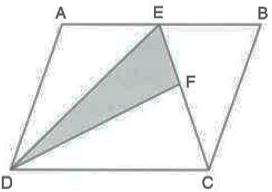
\includegraphics[width=0.4\linewidth]{image.png}
    \end{center}
    \begin{options}
        \item 30
        \item 42
        \item 36
        \item 24
    \end{options}
\end{questionbox}

% Masala 28
\begin{questionbox}{28}
    ABC teng yonli uchburchakda asos AC = 15 va \(\angle BAC = 30^\circ\). AC asosidagi ixtiyoriy M nuqtadan yon tomonlarga perpendikulyarlar tushirilgan. Bu perpendikulyarlar uzunliklari yig'indisini toping.
    \begin{options}
        \item 5
        \item \(\frac{15\sqrt{3}}{2}\)
        \item 7.5
        \item 10
    \end{options}
\end{questionbox}

% Masala 29
\begin{questionbox}{29}
    ABC uchburchakning AB, BC va CA tomonlarida mos ravishda M, N va P nuqtalari olingan, bunda AM:AB = BN:BC = CP:CA = 1:3. MNP uchburchak yuzi 2 ga teng. ABC uchburchak yuzini toping.
    \begin{options}
        \item 7
        \item 5
        \item 4
        \item 6
    \end{options}
\end{questionbox}

% Masala 30
\begin{questionbox}{30}
    Rasmda berilgan ma'lumotlarga ko'ra, \(\angle DTF = x\) burchakning gradus o'lchovini toping.
    \begin{center}
        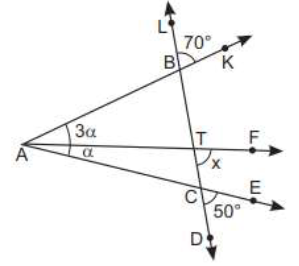
\includegraphics[width=0.5\linewidth]{a.png}
    \end{center}
    \begin{options}
        \item 55
        \item 60
        \item 65
        \item 75
    \end{options}
\end{questionbox}

% Masala 31
\begin{questionbox}{31}
    Rasmda berilgan ma'lumotlarga ko'ra (AB=AC), \(|CD| = x\) kesma uzunligini (sm da) toping.
    \begin{center}
         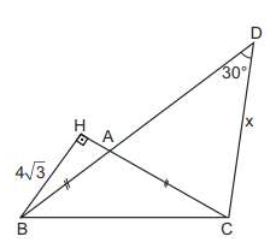
\includegraphics[width=0.4\linewidth]{aa.png}
    \end{center}
    \begin{options}
        \item 8
        \item \(6\sqrt{3}\)
        \item 12
        \item \(8\sqrt{3}\)
    \end{options}
\end{questionbox}

% Masala 32
\begin{questionbox}{32}
    ABC uchburchakda \(\angle ABC = 50^\circ\) va \(\angle ACB = 70^\circ\). Agar AD balandlik, AE esa bissektrisa bo'lsa, \(\angle DAE\) ni toping.
    \begin{options}
        \item \(10^\circ\)
        \item \(15^\circ\)
        \item \(20^\circ\)
        \item \(25^\circ\)
    \end{options}
\end{questionbox}

% Masala 33
\begin{questionbox}{33}
   \(ABCD\) to'gri burchakli trapetsiyada \(AD=8, \ DC = 6, \ BD = 12\) va \(CE\perp BD\) bo'lsa \(|CE|=x-?\)
    \begin{center}
        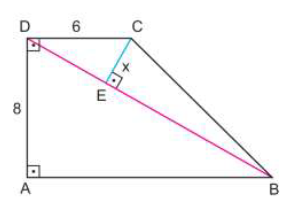
\includegraphics[width=0.5\linewidth]{ddx.png}
    \end{center}
    \begin{options}
        \item \(4\)
        \item \(3\sqrt{2}\)
        \item \(2\sqrt{5}\)
        \item \(2\sqrt{6}\)
    \end{options}
\end{questionbox}

% Masala 34
\begin{questionbox}{34}
    Berilgan ma'lumotlarga ko'ra, ABCD to'rtburchak yuzini (kvadrat birliklarda) toping. $d: y=\frac{3}{5}x+n$ to'g'ri chiziq, B(10,k)
    \begin{center}
       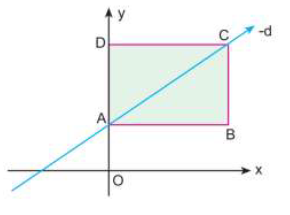
\includegraphics[width=0.5\linewidth]{s.png}
    \end{center}
    \begin{options}
        \item 72
        \item 60
        \item 56
        \item 48
    \end{options}
\end{questionbox}

% Masala 35
\begin{questionbox}{35}
    Agar \(\overline{7x142}\) besh xonali son 11 ga bo'lganda 2 qoldiq qolsa, \(x\) ni toping.
    \begin{options}
        \item 1
        \item 2
        \item 3
        \item 4
    \end{options}
\end{questionbox}

\end{document}